\imageslide{add3.pdf}

%\begin{frame}[fragile]
%\begin{haskellcode}
%data Perhaps a = Unknown | Known a | Contradiction
%\end{haskellcode}
%\end{frame}

\begin{frame}[fragile]

\begin{haskellcode}
data Perhaps a = Unknown | Known a | Contradiction
\end{haskellcode}

\pnl

\begin{haskellcode}
instance Eq a => BoundedJoinSemiLattice (Perhaps a) where

  bottom = Unknown

  (\/) Unknown x           = x
  (\/) x       Unknown     = x
  (\/) Contradiction _     = Contradiction
  (\/) _     Contradiction = Contradiction
  (\/) (Known a) (Known b) =
    if a == b
      then Known a
      else Contradiction
\end{haskellcode}

\end{frame}

\imageslide{perhaps1.pdf}
\imageslide{perhaps2.pdf}


%\imageslideleft{contradiction4.pdf}
%\imageslideleft{contradiction5.pdf}
%\imageslideleft{contradiction6.pdf}
%\imageslideleft{contradiction7.pdf}
%\imageslideleft{contradiction8.pdf}
%\imageslideleft{contradiction9.pdf}
\imageslide[0.6]{doubleplus0.pdf}
\imageslide[0.6]{doubleplus1.pdf}
\imageslide[0.6]{doubleplus2.pdf}
%\imageslide[0.6]{doubleplus3.pdf}
\imageslide[0.6]{doubleplus4.pdf}
\imageslide[0.6]{doubleplus5.pdf}
\imageslide[0.6]{doubleplus6.pdf}
\imageslide[0.6]{doubleplus7.pdf}
\imageslide[0.6]{doubleplus8.pdf}


\begin{frame}
\begin{columns}
\column{0.5\textwidth}
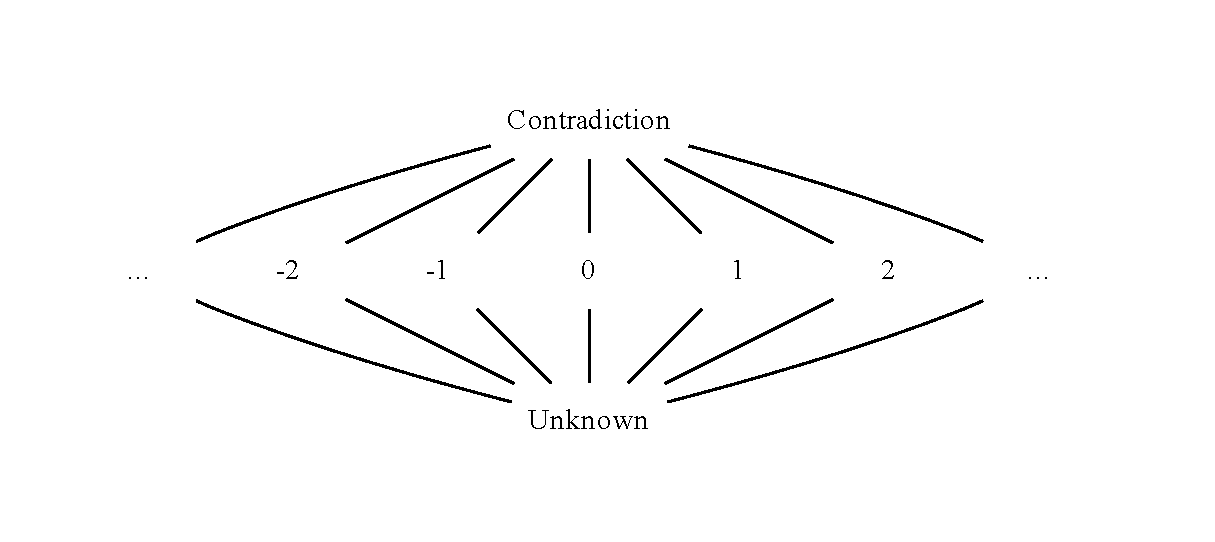
\includegraphics[scale=0.65]{flat.pdf}
\pause
\column{0.2\textwidth}
\column{0.3\textwidth}
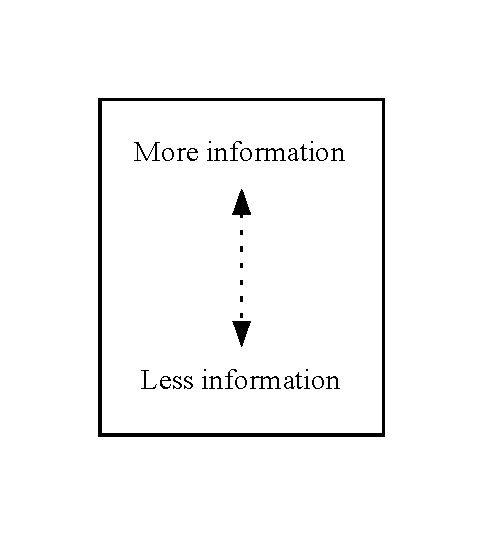
\includegraphics[scale=0.65]{more-information.pdf}
\end{columns}
\end{frame}

